% ----------------------------------------------------------------------

\newpage

\subsection{\iv Test}
\label{ss:iv}

\subsubsection{Purpose}

The \iv test is unique in that it doesn't directly utilize the read-out functionality of the \roc.
In fact, this test can be performed on a sensor before it's even bump-bonded onto a set of \rocs.
In principle, the silicon sensor acts like a diode, 
allowing current to flow in the ``forward'' direction but not in the ``reverse'' direction.
A potential difference is created across the sensor, in the plane transverse to the sensor face,
by applying a ``reverse bias'' voltage.
This potential difference is what draws the electrons created by a charged particle passing through the sensor 
towards the bump-bond to be collected.
For a given sensor, the reverse bias has an operating range.
If the bias is too small, the sensor will not be depleted of free electrons and will not operate properly.
If the bias is too large, the sensor will break down and start acting like a resistor instead of a diode.
The \iv test is meant to determine the operating range of the sensor, 
bounded by the depletion voltage (lower limit) and the breakdown voltage (upper limit).

\subsubsection{Methodology}

This test is exceedingly simple, it merely performs a scan over a range of bias voltages
and records the current draw of the system at each point.
During the test, control is taken over the HV supply in order to effect a voltage sweep.
The user can configure the range of voltages to scan (default is 0V-600V),
the step size between measurements (default 10V), 
and the amount of time between measurements to allow the system to react to the voltage change (default is 1s).
To protect the module from damage due to excessively high voltages, a compliance current is set (default is 100 $\mu$A).
If the current reaches this compliance level, the scan is aborted and the voltage turned off.
The single output from this test is a plot of the current draw as a function of the bias voltage
as shown in Figure~\ref{fig:iv_IVcurve}.
The module in question has an operating plateau from roughly -100V to -200V.

\subsubsection{Output}

\begin{figure}[!htp]
\centering
\begin{minipage}{0.45\textwidth}
  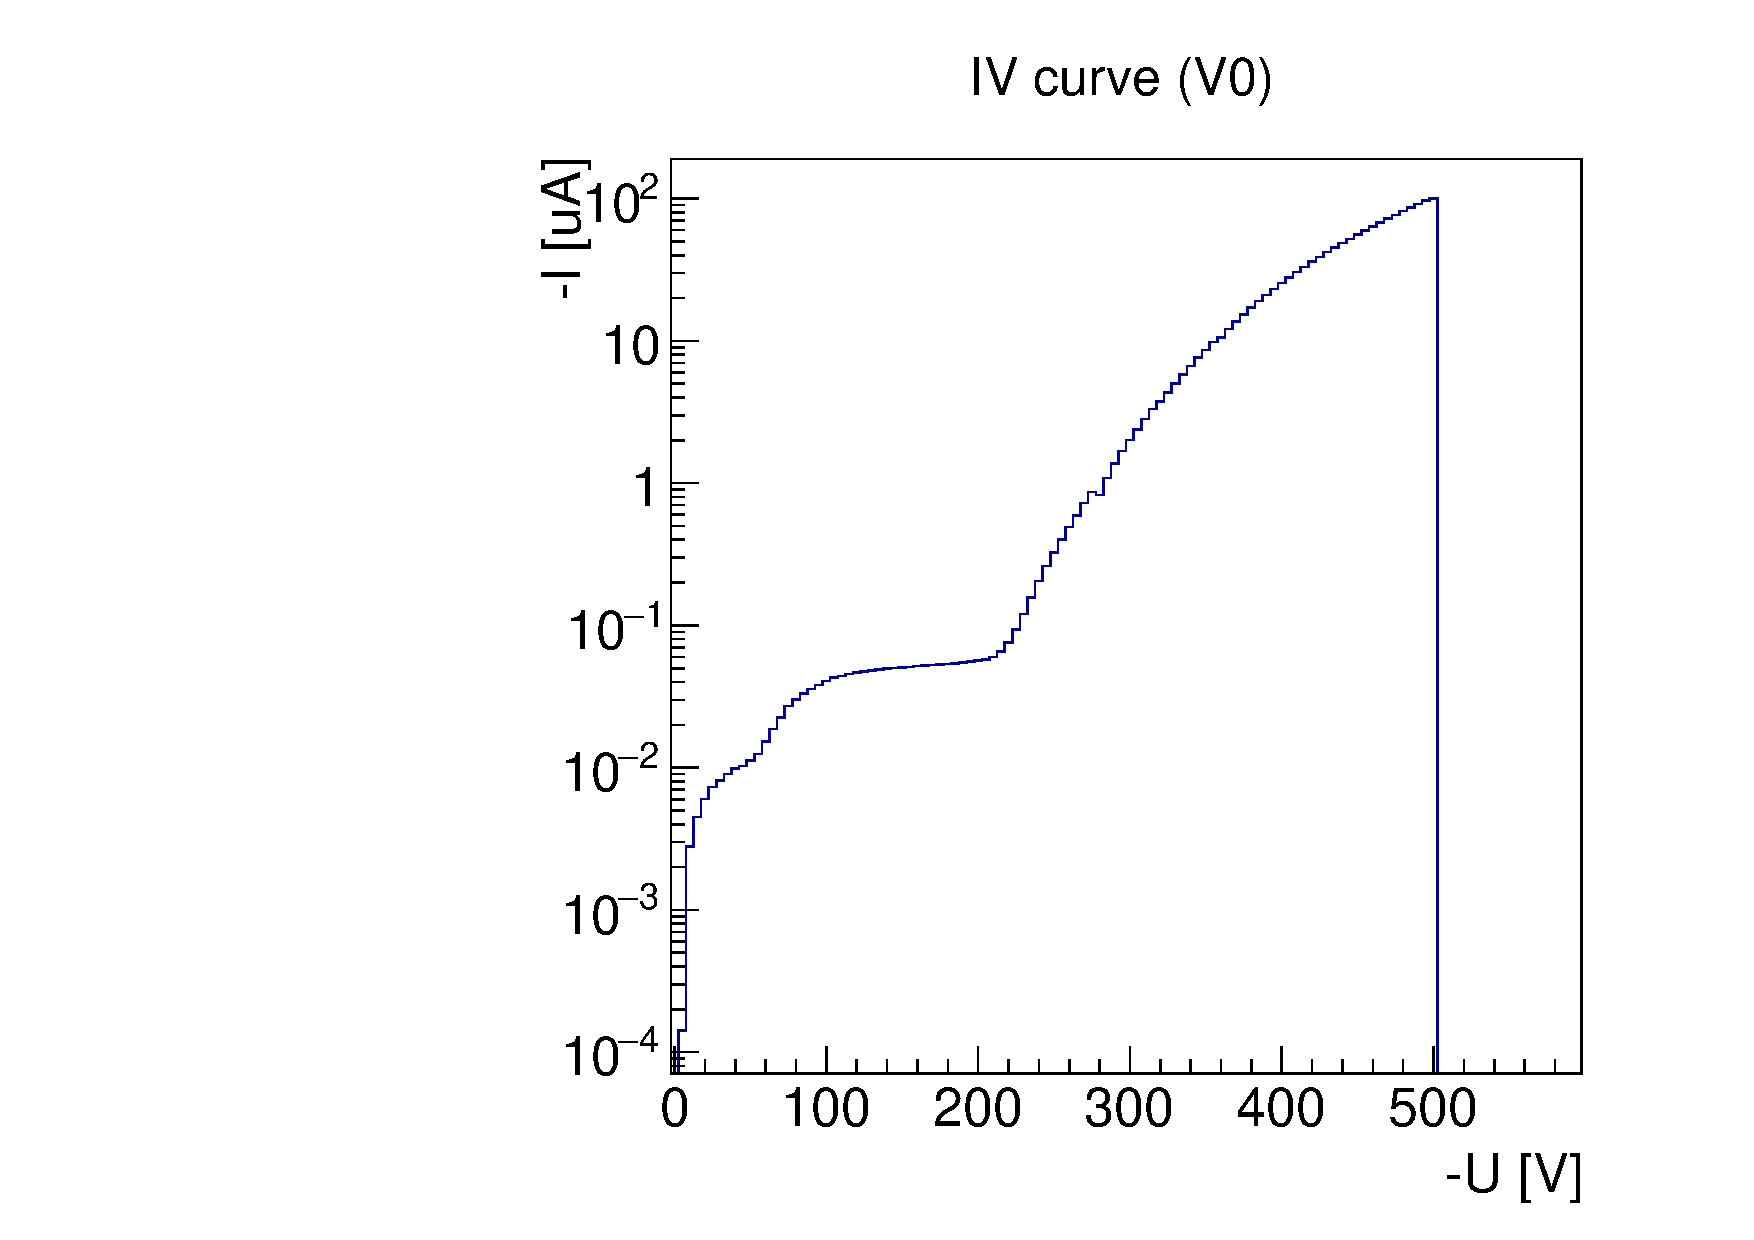
\includegraphics[width=1.0\textwidth]{figures/iv_IVcurve.pdf}
  \caption{Current draw in the module as a function of (reverse) bias voltage.
The module shown is fully depleted by -100V and shows a breakdown voltage near -200V.}
  \label{fig:iv_IVcurve}
\end{minipage}
\end{figure}
